\chapter[Fundamentação Teórica]{Fundamentação Teórica}


\section{Modelo físico}

Neste trabalho, procura-se analisar o perfil térmico sobre um escoamento turbulento no canal de Poiseuille. Ele pode ser definido como um escoamento confinado entre duas placas infinitas. Nelas, o escoamento atinge velocidade igual a zero (condição de não deslizamento) e estão em regime de fluxo térmico constante. Tais placas encontram-se perpendiculares ao eixo $y$. O eixo $z$ é definido como auto-similar tanto na velocidade quanto na temperatura, resultando em um domínio plano (Fig.\ref{descricaoGeometrica}). O escoamento foi considerado incompressível e o fluido foi considerado newtoniano. Neste sistema físico, o fluido escoa, em média, somente na direção do eixo $x$.
Os números de Reynolds ($Re = \frac{2R \overline{U}}{\nu}$) variam de $4560$ a $41441$, resultando em um regime turbulento.

\begin{figure}[h!]
	\centering
	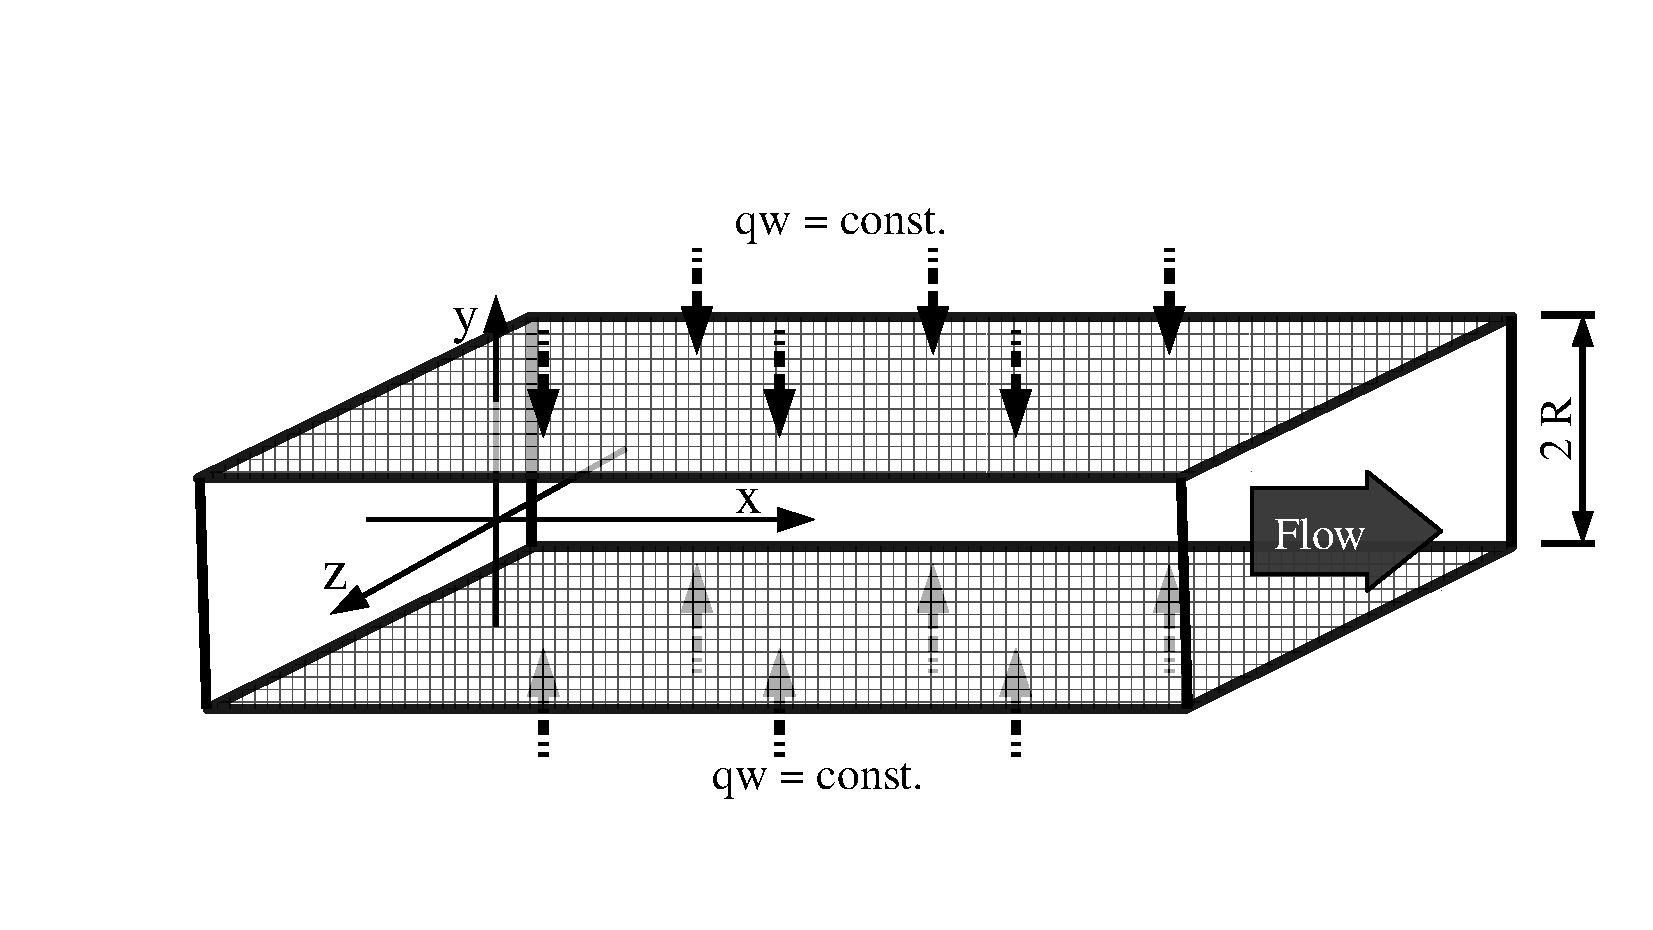
\includegraphics[angle=0, trim={0mm 23mm 0mm 35mm}, clip , scale=0.42]{cap_fundamentacao/canal1.pdf}
	\caption{Definição geométrica e condições de contorno.}
  \legend{Fonte: Autor.}
	\label{descricaoGeometrica}
\end{figure}

Estas foram as suposições efetuadas para o problema proposto, que serão consideradas no modelo matemático diferencial adiante.

\section{Modelo matemático diferencial}
A formulação matemática do problema foi baseada nas equações de continuidade, de Navier-Stokes \cite{Cengel}, e na equação de transporte de energia térmica \cite{Incropera}: 

\begin{equation}
  \frac{\partial u}{\partial t} + \frac{\partial u^2}{\partial x} + \frac{\partial uv}{\partial y} + \frac{\partial uw}{\partial z} = - \frac{1}{\rho} \frac{\partial {p}}{\partial x} + \nu \left( \frac{\partial^2 u}{\partial x^2} + \frac{\partial^2 u}{\partial y^2} + \frac{\partial^2 u}{\partial z^2}   \right)
\end{equation}

\begin{equation}
  \frac{\partial \rho}{\partial t} +  \frac{\partial (\rho u)}{\partial x} + \frac{\partial (\rho v)}{\partial y} + \frac{\partial (\rho w)}{\partial z} = 0
\end{equation}

\begin{equation}
  \frac{\partial T}{\partial t} + {\frac{\partial{}}{\partial{x}} (uT)} + {\frac{\partial{}}{\partial{y}} (vT)} + {\frac{\partial{}}{\partial{z}} (wT)}
  =
  {\frac{\partial{}}{\partial{x}}} \left(\alpha {\frac{\partial{T}}{\partial{x}}} \right) +
  {\frac{\partial{}}{\partial{y}}} \left(\alpha {\frac{\partial{T}}{\partial{y}}} \right) +
  {\frac{\partial{}}{\partial{z}}} \left(\alpha {\frac{\partial{T}}{\partial{z}}} \right)
\end{equation}

\begin{equation}\label{resfriamentoDeNewton}
  q_{conv.} = \dot{m} C_p \Delta T_m.
\end{equation}

Eq.\ref{resfriamentoDeNewton} é baseada na lêi de resfriamento de newton \cite{Incropera}, onde $\dot{m}$ é a vazão volumétrica, $C_p$ é a capacidade calorífica específica, $\Delta T_m$ é a diferença de temperatura entre a superfície e o fluido, e $q_{conv.}$ é a taxa de transferência de calor por convecção.

\subsection{O estudo dos comportamentos médios}
Para simplificar o sistema, foi realizado um tratamento estatístico nas equações. Cada grandeza foi dividida entre valor médio e flutuações, sendo que a média torna-se independente do tempo:

\begin{equation}
  \overline{f}({x})=\frac{1}{t_f - t_i} \int_{t_i}^{t_f} f({x} , t) dt.
\end{equation}

\begin{equation}
  f({x} , t) = \overline{f}({x}) + f^\prime ({x} ,t),
\end{equation}

também é possível realizar as seguintes operações com as flutuações:

\begin{equation}
  \begin{cases}
  \overline{f^\prime ({x} ,t)} = 0 , & \quad   \\
  \overline{\overline{f({x})}} = \overline{f({x})} , & \quad   \\
  \overline{f^\prime ({x} ,t)\overline{f({x})}} = 0 ,& \quad   \\
  \overline{f^\prime ({x} ,t)g^\prime ({x} ,t)} \neq 0 , & \quad   \\
  \overline{  \overline{g({x})} \ \overline{f({x})}  } = {\overline{g({x})}} \ {\overline{f({x})}} , & \quad   \\
  \end{cases}
\end{equation}

A partir destas operações foi possível simplificar o sistema de equações. É possível se representar geométricamente também essa separação entre a média e flutuação na Figura \ref{figura.1}:

\begin{figure}[h!]
	\centering
	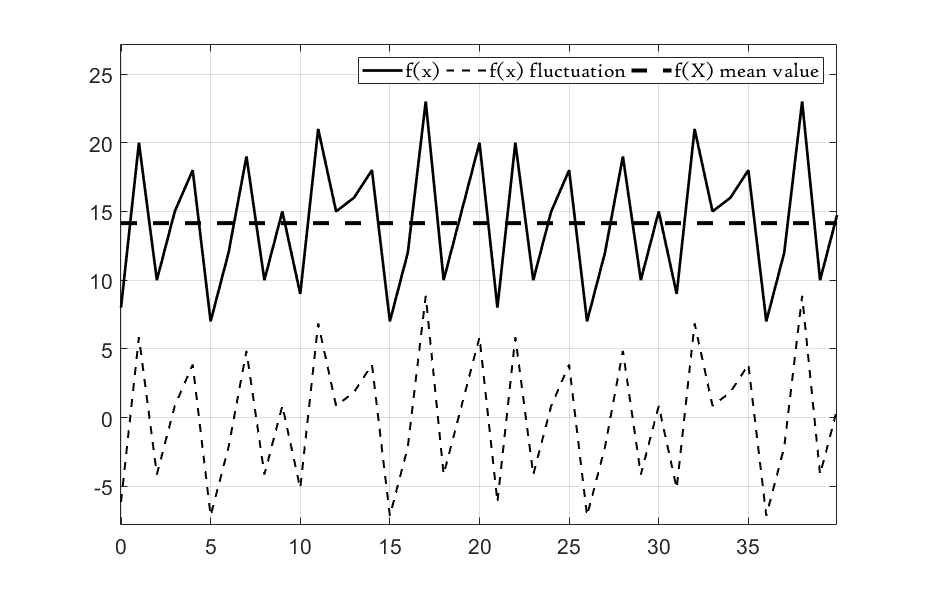
\includegraphics[angle=0, scale=0.60]{medios}
	\caption{Representação geométrica da separação entre os valores médios e as flutuações.}
  \legend{Fonte: Autor.}
	\label{figura.1}
\end{figure}

Dessa forma, aplicando as simplificações, obtêm-se as equações médias da continuidade (Eq.\ref{mass}), de Navier-Stokes (Eq.\ref{dynamics}) e de balanço de energia (Eq.\ref{energy permanent}):

\begin{equation}\label{mass}
\frac{\partial \overline{u}}{\partial x} = 0,
\end{equation}

\begin{equation}\label{dynamics}
\frac{\partial \overline{u} \, \overline{v}}{\partial y} = 
- \frac{1}{\rho} \frac{\partial \overline{p}}{\partial x} + \frac{\partial}{\partial y}\left(\nu \frac{\partial \overline{u}}{\partial y} - \overline{u^\prime v^\prime}\right),
\end{equation}


\begin{equation}\label{energy permanent}
\frac{\partial{}}{\partial{x}} \left(\overline{T^\prime u^\prime}\right) + \frac{\partial{}}{\partial{x}}\left(\overline{u} \overline{T}\right)     + 
\frac{\partial{}}{\partial{y}} \left(\overline{T^\prime v^\prime}\right) + \frac{\partial{}}{\partial{y}}\left(\overline{v} \overline{T}\right) 
=
{\frac{\partial{}}{\partial{x}}} \left(\alpha {\frac{\partial{\overline{T}}}{\partial{x}}} \right) +
{\frac{\partial{}}{\partial{y}}} \left(\alpha {\frac{\partial{\overline{T}}}{\partial{y}}} \right). 
\end{equation}

Sendo $\overline{u}$ e $\overline{v}$ as velocidades médias e $u^\prime$ e $v^\prime$ as flutuações na velocidade nos eixos $x$ e $y$, $\rho$ a massa específica, $\overline{p}$ a pressão média, $\nu$ a viscosidade cinemática, $\overline{T}$ a temperatura média, $T^\prime$ a flutuação na temperatura e $\alpha$ a difusividade térmica.

O método, independente da variável do tempo e baseado em comportamentos médios, é caracterizado como um exemplo de metodologia RANS (Reynolds-averaged Navier-Stokes).


\subsection{O regime permanente térmico}

O campo de velocidade média atinge regime estatisticamente permanente no canal (Fig. \ref{figure.3}), mas o mesmo não ocorre para o campo de temperatura, pois um fluxo térmico constante é imposto sobre as paredes. A temperatura continua aumentando no domínio, nunca se estabilizando.
Outra diferença entre os dois domínios é o fato de que o perfil de velocidade mantém-se constante no sentido do fluxo. Isso possibilita que o sistema seja representado unidimensionalmente, simplificando drasticamente as formulações matemáticas. O mesmo não pode ser dito para o campo de temperatura média, as temperaturas aumentam linearmente no sentido do fluxo (Fig. \ref{figure.2}):

\begin{figure}[h!]
	\centering
	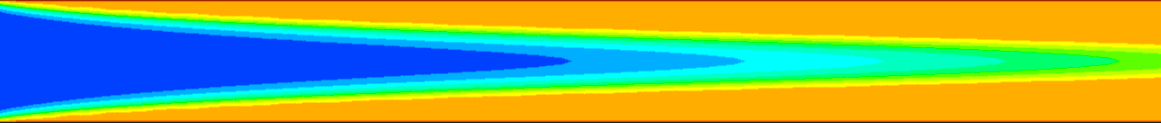
\includegraphics[angle=0, scale=0.4]{cap_fundamentacao/temperatura.png}
	\caption{Campo de temperatura média no canal de Poiseuille. O perfil de temperatura no canal aumenta linearmente na direção do fluxo.}
  \legend{Fonte: Autor, em simulação realizada no Mfsim.}
	\label{figure.2}
\end{figure}
\begin{figure}[h!]
	\centering
	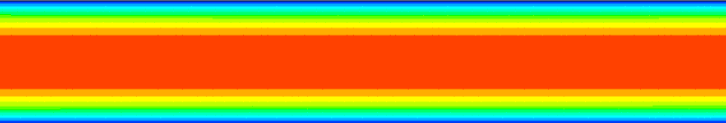
\includegraphics[angle=0, height=1.35cm , width=12.3cm]{cap_fundamentacao/velocidade.png}
	\caption{Campo de velocidade média no canal de Poiseuille. O perfil se mantém constante na direção do fluxo.}
  \legend{Fonte: Autor, em simulação realizada em código próprio.}
	\label{figure.3}
\end{figure}

Para simplificar o equacionamento do campo de temperatura médio, um balanço de energia térmica foi estudado (Eq. \ref{c_h_e}):

\begin{equation}\label{c_h_e}
q_{conv.} = \dot{m} C_p \Delta T_m,
\end{equation}

A partir da equação de balanço de energia térmica, pode-se obter a temperatura média no domínio:

\begin{equation}
2q_w b \Delta x = \dot{m} C_p \Delta T_m,
\end{equation}\\

\begin{equation}
\Delta T_m = \frac{2q_w b \Delta x}{\dot{m} C_p},
\end{equation}

Onde $q_w$ é o fluxo de calor nas paredes, $b$ é a largura do canal e $\Delta x$ é a distância entre as paredes.\\
Então, subistituindo $ \dot{m} = u_m 2R b \rho $ onde $u_m$ é a velocidade média no domínio, $R$ é o raio do canal e $\rho$ é a massa específica, e se assumindo que $ \Delta T_m = \frac{\partial{\left(\overline{T}_m\right)}}{\partial{x}} \Delta x $: 

\begin{equation}\label{c_h_ee}
\frac{\partial{\left(\overline{T}_m\right)}}{\partial{x}} = \frac{q_w}{u_m R \rho C_p}.
\end{equation}

Como todos os termos à direita da equação são constantes, a temperatura média varia linearmente no sentido da corrente.\\
Para melhor entender a temperatura nas paredes, uma formulação de convecção termal foi estudada:

\begin{equation}
q_w = h A \left( T_w(x) - \overline{T}_m(x)\right).
\end{equation}

Como se tem um fluxo completamente desenvolvido, pode-se afirmar que o valor de $h$ é constante. Assim, usando-se a Eq. \ref{c_h_ee}, é possível se concluir que:

\begin{equation}
\frac{d T_w(x)}{d x} = \frac{d \overline{T}_m(x)}{d x} = Cte.
\end{equation}	

Dessa forma, considerando que a temperatura nas paredes varia linearmente, assim como a temperatura média, é possível se extender esse gradiente no domínio completo ao se considerar as condições de contorno e a simetria do systema. Assim, nas paredes é imposto um gradiente de temperatura constante, criando-se um regime de condição de contorno de fluxo térmico constante. Consequentemente, todo o campo de temperatura varia linearmente na direção da corrente e com o tempo.
O valor de temperatura foi então decomposto no seguinte modo:

\begin{equation}
   T^\ast(y) = T(x,y) - T_w(x),
\end{equation}


 Onde $T^\ast(y)$ é a temperatura relativa, $T(x,y)$ é a temperatura absoluta e $T_w(x)$ é a temperatura na parede.\\

 Assim, analisando-se $T^\ast(Y)$, vemos auto-similaridade no sentido da corrente, resultando em um equacionamento unidimentional representativo com solução em $T^\ast(y)$.

 Finalmente Eq. \ref{energy permanent}:

\begin{equation}
\begin{split}
\frac{\partial{}}{\partial{x}} \left(\overline{(T^\ast + T_w)^\prime} \overline{ u^\prime}\right) + \frac{\partial{}}{\partial{x}}\left(\overline{(T^\ast + T_w)} \overline{u}\right)+ 
\frac{\partial{}}{\partial{y}} \left(\overline{(T^\ast + T_w)^\prime} \overline{ v^\prime}\right) + \frac{\partial{}}{\partial{y}}\left(\overline{(T^\ast + T_w)} \overline{v}\right) = \\
{\frac{\partial{}}{\partial{x}}} \left(\alpha {\frac{\partial{\overline{(T^\ast + T_w)}}}{\partial{x}}} \right) +
{\frac{\partial{}}{\partial{y}}} \left(\alpha {\frac{\partial{\overline{(T^\ast + T_w)}}}{\partial{y}}} \right). 
\end{split}
\end{equation}

Então a expressão pode ser desenvolvida ainda mais algebricamente considerando todas as velocidades médias nas direções $y$ e $z$ nulas:

\begin{equation}\label{equation_var}
{\frac{\partial{}}{\partial{y}}} \left(\alpha {\frac{\partial{\overline{T^\ast}}}{\partial{y}}}   
- \left(\overline{ T^{\ast\prime} v^\prime}\right) \right)
= 
\overline{u}\frac{\partial{\overline{T_w}}}{\partial{x}}.
\end{equation}

\subsection{A hipótese de Bousinesq}

A hipótese de Bousinesq é uma aproximação que permite a análise de sistemas de convecção térmica em regime permanente. No caso do presente trabalho a hipótese foi empregada no termo $\overline{T^{\ast\prime}  v^\prime}$, que pode, então, ser modelado como segue:

\begin{equation}\label{bou}
-\left(\overline{ T^{\ast\prime}  v^\prime}\right) = 
\alpha_t \frac{\partial{\overline{T^\ast}}}{\partial{y}}.
\end{equation}

Onde $\alpha_t$ é a difusividade térmica turbulenta do fluido. Assim, substituindo-se Eq. \ref{bou} na Eq. \ref{equation_var}:

\begin{equation}\label{oiiiii}
{\frac{\partial{}}{\partial{y}}} \left[(\alpha + \alpha_t)  \frac{\partial \overline{T^\ast}}{\partial y} \right]
= 
\overline{u}\frac{\partial{\overline{T_w}}}{\partial{x}}. 
\end{equation}

\subsection{O comprimento de mistura de Prandtl}

O termo da difusão térmica turbulenta, $\alpha_t$, precisa ser modelado. Para modelá-lo, usou-se o conceito clássico do número de prandtl turbulento que é:

\begin{equation}
Pr_t = \frac{\nu_t}{\alpha_t}.
\end{equation} 

A viscosidade cinemática turbulenta $\nu_t$ precisa ser modelada. O valor do número de prandtl turbulento pode ser definido como $Pr_t = 0.71$, como consta na literatura.

Com o modelo de comprimento de mistura de Prandtl, é definido:

\begin{equation}
\nu_t = {l^2_m} \left| \frac{\partial \overline{u}}{\partial y} \right|.
\end{equation}

\begin{equation}\label{3332x}
\alpha_t = \frac{{l^2_m}}{Pr_t} \left| \frac{\partial \overline{u}}{\partial y} \right|.
\end{equation}

Onde $l_m$ é o comprimento de mistura. Então substituindo-se Eq. \ref{3332x} na Eq. \ref{oiiiii}:

\begin{equation}\label{equationquasela}
{\frac{\partial{}}{\partial{y}}} \left( \left( \alpha   
+ \frac{{l^2_m} \left| \frac{\partial \overline{u}}{\partial y} \right|}{Pr_t} \right) \frac{\partial \overline{T^\ast}}{\partial y} \right)
= 
\overline{u}\frac{\partial{}}{\partial{x}}\left(\overline{T_w}\right)  .
\end{equation}

É possível notar, quando se analisa a dinâmica do fluido, que para valores positivos de $y$, a derivada da velocidade é sempre negativa, com uma velocidade que decresce com y. Resultando em:

\begin{equation}
{\frac{\partial{}}{\partial{y}}} \left( \left( \alpha   
- \frac{{l^2_m}}{Pr_t}\frac{\partial \overline{u}}{\partial y} \right) \frac{\partial \overline{T^\ast}}{\partial y} \right)
= 
\overline{u}\frac{\partial{}}{\partial{x}}\left(\overline{T_w}\right)  .
\end{equation}

\subsection{O comprimento de mistura}

O comprimento de mistura $ l_m $ precisa ser modelado. Os estudos experimentais de nikuradse foram usados para modelar esse parâmetro para escoamentos de canal, como segue:

\begin{equation}
L\left(\frac{y}{R}\right) = \frac{l_m}{R} = 0.14 - 0.08 \left(\frac{y}{R}\right)^2 - 0.06\left(\frac{y}{R}\right)^4.
\end{equation}

Para maior completude do modelo, cebeci e bradshaw adicionaram a função de amortecimento de Van Driest:

\begin{equation}\label{eqution_mixturelength}
L\left(\frac{y}{R}\right)  = \frac{l_m}{R} = \left\{ 0.14 - 0.08 \left(\frac{y}{R}\right)^2 - 0.06\left(\frac{y}{R}\right)^4\right\}\left\{  1 - e^{[(\frac{y}{R} - 1) \frac{Re_\tau}{A}]}\right\},
\end{equation}

Com $A = 26$ como a constante de Cebeci. Assim, tem-se o comprimento de mistura definido como:

\begin{equation}
l_m = L R,
\end{equation}

Sendo $L$ uma função no eixo $y$, dado pela equação \ref{eqution_mixturelength}. Então a equação \ref{equationquasela} pode ser escrita da seguinte forma:

\begin{equation}\label{cebeciconstant}
{\frac{\partial{}}{\partial{y}}} \left( \left( \alpha   
- \frac{{L}^2 R ^2}{Pr_t}\frac{\partial \overline{u}}{\partial y} \right) \frac{\partial \overline{T^\ast}}{\partial y} \right)
= 
\overline{u}\frac{\partial{}\left(\overline{T_w}\right)  }{\partial{x}}.
\end{equation}

Usando-se coordenadas de parede, a equação foi adimensionalizada, para que pudesse ser comparada com a literatura. As considerações adotadas foram: $ \tilde{y} = \frac{y . Re_\tau}{R} $, $ \tilde{\overline{u}} = \frac{\overline{u}}{u_\tau} $ , $ \tilde{\overline{T}} = \frac{\overline{T}}{T_\tau} $ , $ \tilde{\overline{T^\ast}} = \frac{\overline{T^\ast}}{T_\tau} $ , $Re_\tau = \frac{u_\tau R}{\nu}$, $Pr_t = \frac{\nu_t}{\alpha_t}$, $Pr = \frac{\nu}{\alpha}$, $T_\tau = \frac{q_w}{\rho C_p u_\tau}$, $\frac{\partial{\left(T_m\right)}}{\partial{x}} = \frac{q_w}{u_m  R \rho  C_p } $ e $\frac{\partial \overline{p}}{\partial x} = - \frac{u_\tau^2 \rho}{R} $. Que, ao se substituir em (\ref{cebeciconstant}) resultou em (\ref{equationultima}):
\\
\begin{equation}\label{equationultima}
{\frac{\partial{}}{\partial{\tilde{y}}}} \left( \left( \frac{Re_\tau}{Pr}   
- \frac{{L}^2 Re_\tau ^3}{Pr_t}\frac{\partial \tilde{\overline{u}}}{\partial \tilde{y}} \right) \frac{\partial \tilde{\overline{T^\ast}}}{\partial \tilde{y}} \right)
= 
\frac{\tilde{\overline{u}}}{\tilde{u_m}}.
\end{equation}

É importante observar que existe a velocidade na equação (\ref{equationultima}), ou seja, para o desenvolvimento do problema térmico é necessário o desenvolvimento do perfil dinâmico do canal. Para isso, foi utilizada uma metodologia rans previamente estabelecida \cite{luigi}, conforme segue:

\begin{equation}\label{finalequationvelocity}	
\frac{\partial \tilde{\overline{u}}}{\partial \tilde{y}} = - \frac{2 \tilde{y} \frac{1}{Re_\tau} }{ 1 + \sqrt{ 1 + 4 L ^2 Re_\tau ^2 \tilde{y}}}.
\end{equation}	

Assim, tem-se a primeira derivada da velocidade determinada algebricamente.

\newpage

\section{Modelo matemático numérico}

Para discretizar a equação diferencial, um domínio euleriano foi declarado. Para a velocidade foi aplicado um método runge-kutta de quarta ordem, enquanto a temperatura foi arranjada em um esquema de diferenças centradas que teve que ser resolvido implicitamente.
O modelo dinâmico é resolvido primeiro, e seu resultado é usado na solução do perfil térmico. O centro da célula foi usado de forma que a parede fosse colocada no centro da célula e um ponto entre as células fosse colocado no ponto central do canal. A convergência dos resultados numéricos é mostrada na figura \ref{sistema}:

\begin{figure}[!h]
	\centering
	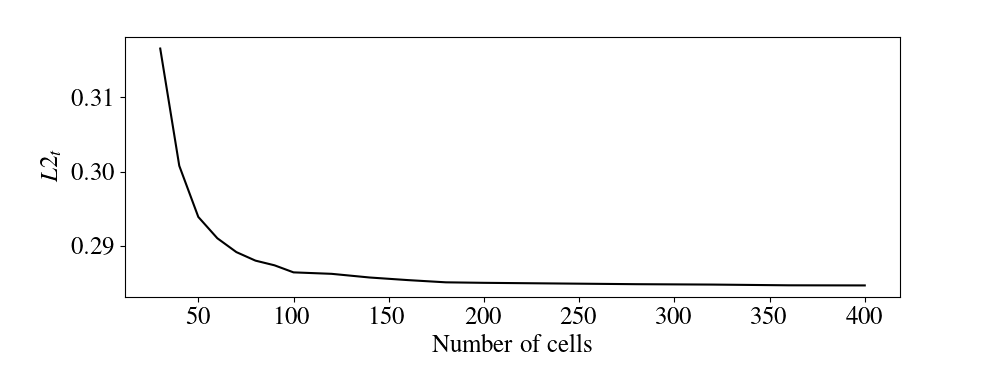
\includegraphics[angle=0, trim={10mm 0mm 0mm 0mm}, clip , scale=0.50]{fotos_formatacao_final/Convergence}
	\caption{Norma L2 de simulação térmica comparado a dns até 400 células, com $Re_\tau = 1020$.}
	\label{sistema}
\end{figure}

Quanto maior o número de elementos na malha, maior a acurácia do resultado até atingida a convergência quando comparado aos resultados em DNS. A partir disso, os erros observados deixam de ser devido ao método numérico e têm significância quanto aos ajustes aplicados, como, por exemplo, a hipótese de bousinesq.

Dessa forma, para cada resultado, deu-se um número suficiente de elementos para que houvesse a convergência do erro numérico.


\chapter{Ajustes propostos}

\subsection{Resultados via método canônico}
Inicialmente o número de prandtl turbulento, $Pr_t = 0,71$, foi usado como na literatura. Os resultados obtidos apresentados na figura \ref{figuraresultados1} são comparados com os dns de \cite{dns1020} e \cite{dns150}, com a norma l2.\\

\begin{figure}[!h]
  \centering
  \begin{minipage}{0.49\textwidth}
    \centering
    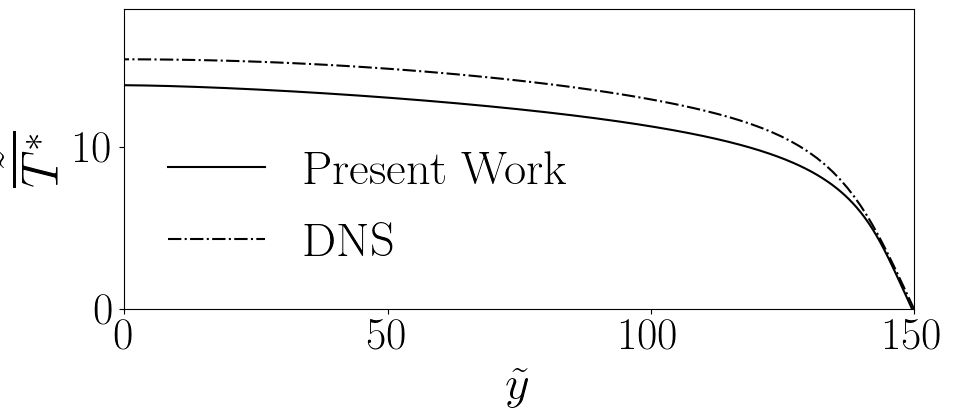
\includegraphics[angle=0, scale=0.32]{fotos_formatacao_final/Temperature_150_071_classico}
    \subcaption{$Re_\tau = 150$, $L2_t = 1.42$}
  \end{minipage}
  \hfill
  \begin{minipage}{0.49\textwidth}
    \centering
    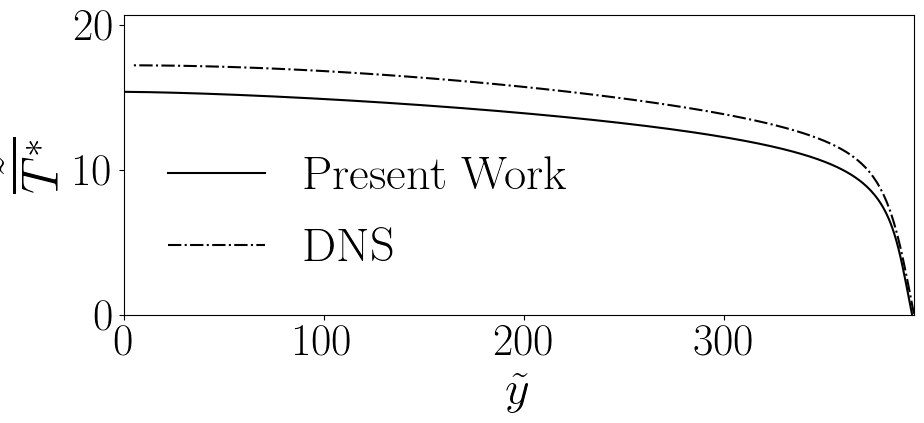
\includegraphics[angle=0, scale=0.32]{fotos_formatacao_final/Temperature_395_071_classico}
    \subcaption{$Re_\tau = 395$, $L2_t = 1.55$}
  \end{minipage}
  \begin{minipage}{0.49\textwidth}
    \centering
    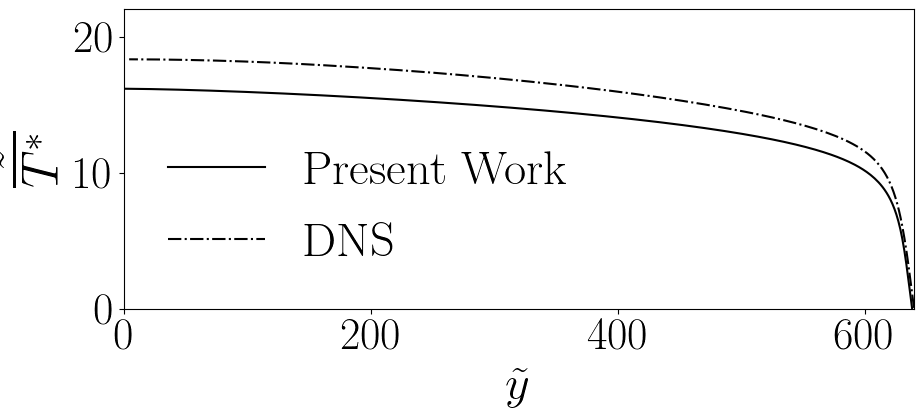
\includegraphics[angle=0, scale=0.32]{fotos_formatacao_final/Temperature_640_071_classico}
    \subcaption{$Re_\tau = 640$, $L2_t = 1.79$}
  \end{minipage}
  \hfill
  \begin{minipage}{0.49\textwidth}
    \centering
    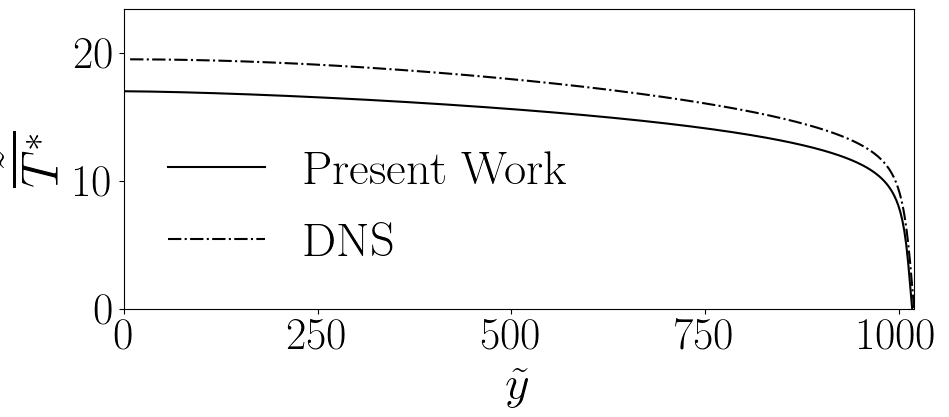
\includegraphics[angle=0, scale=0.32]{fotos_formatacao_final/Temperature_1000_071_classico}
    \subcaption{$Re_\tau = 1020$, $L2_t = 2.04$}
  \end{minipage}
  \caption{Distribuição de temperatura para $Pr_t = 0.71$, $A = 26$ e $Pr = 0.71$.} 
  \label{figuraresultados1}
\end{figure}

Os primeiros resultados mostram um forte efeito negativo das aproximações empregadas. Percebeu-se que o número de prandtl turbulento teve grande influência no resultado.
A grandeza podia ser encontrada no banco de dados do DNS, e observou-se que ela variava em função da distância da parede (\cite{dns1020} e \cite{dns150}) (figure \ref{figure5}).
O valor então foi extraído do banco de dados e usado como parâmetro durante uma simulação do método descrito no presente trabalho, obtendo-se uma norma L2 de $ 0,19 $ para $ Re_t = 640 $.

Assim foi validado que o problema estava na parametrização do número de prandtl turbulento.

\begin{figure*}[h!]
	\centering
	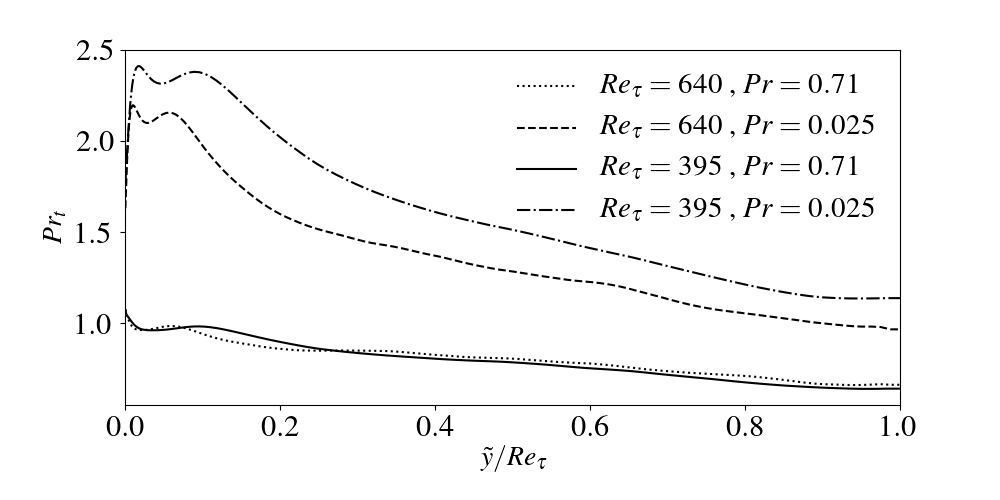
\includegraphics[angle=0, scale=0.62]{fotos_formatacao_final/DNS_PRt}
	\caption{Número de Prandtl turbulento adquirido do DNS em função de $ \tilde{y}/Re_\tau $, a distância até a parede no canal.}
	\label{figure5}
\end{figure*}

Assim, iniciou-se o esforço de propor uma parametrização ajustada para o número de prandtl turbulento. Neste sentido tentou-se ajustar um valor para que o erro fosse mínimo, quando comparado com o DNS. Neste sentido, aplicou-se a metodologia de algoritmos baseados em evolução diferencial \cite{Price2013}.

\subsection{O meta modelo adquirido via evolução Diferencial (DE)}

Foi utilizado um algoritmo de evolução diferencial \cite{diferential} na procura da melhor parametrização possível do Prandtl turbulento. Neste algorítmo, arbitra-se um valor editável pelo algorítmo e uma função objetiva cujo programa tentará minimizar ajustando valores na variável editável. Durante as iterações de simulações, os resultados direcionam o algorítmo, cujas tentativas concentram-se mais e mais ao redor do mínimo encontrado pela função objetiva.

Considerou-se o número de prandtl turbulento como variável livre e a norma L2 como função objetiva.
O erro foi calculado comparando a temperatura resultante com os dados DNS (\cite{dns1020} e \cite{dns150}). Obteve-se um número prandtl turbulento de $ 0.9$, para o número de Reynolds $ Re_\tau = 1020$.

É importante ressaltar que o número de prandtl turbulento foi encontrado como uma constante. Apesar de, nos dados do DNS ele ser apresentado como um vetor de valores em função da distância da parede, optou-se por buscar uma constante representativa, de forma a se simplificar a abordagem.



Pode-se ver adiante a forma como o algorítmo genético evoluiu para encontrar o valor de $ Pr_t $ ideal, ou seja, o valor que resultada no menor erro.

\begin{figure}[!h]
	\centering
	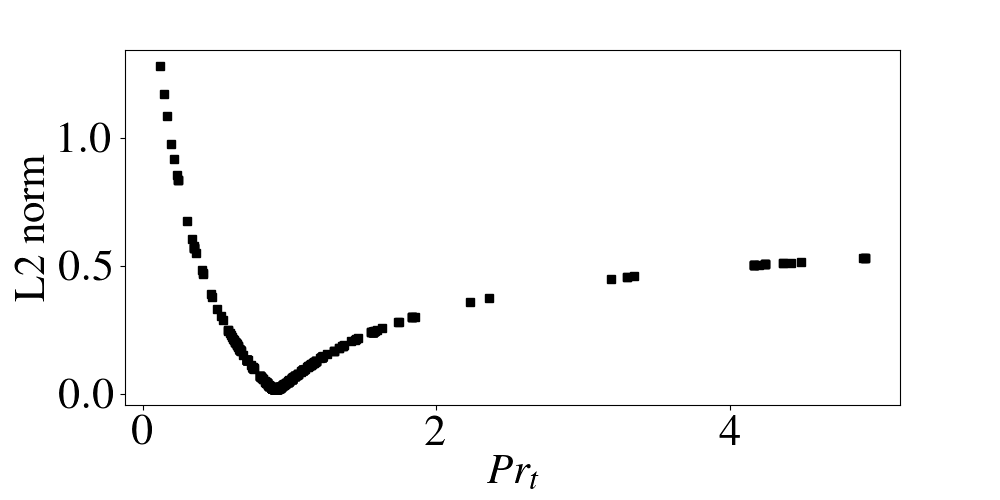
\includegraphics[angle=0, scale=0.61]{fotos_formatacao_final/Genetic_amostra}
	\caption{Iterações de algoritmo genético, com simulações para $Re_\tau = 1020$. Convergência em $Pr_t = 0.9 $.}
\end{figure}

O número de prandtl turbulento obtido, $Pr_t = 0.9$ que minimiza o erro no campo da temperatura, foi considerado aos demais números de Reynolds, resultando na figura \ref{primeiros}.

\begin{figure*}[!h]
	\centering
	\begin{minipage}[t]{0.5\textwidth}
		\centering
		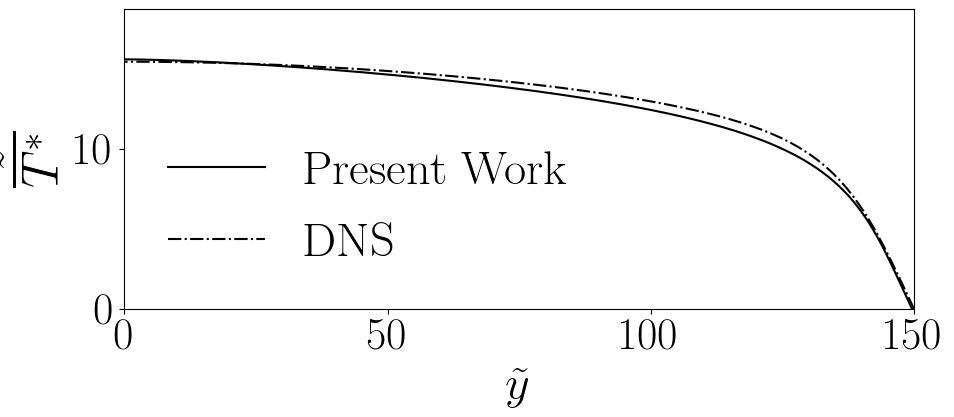
\includegraphics[angle=0, scale=0.34]{fotos_formatacao_final/Temperature_150_071_Prt0905_A26}
		\subcaption{$Re_\tau = 150$, $L2_t = 0.34$}
	\end{minipage}
	\begin{minipage}[t]{0.45\textwidth}
		\centering
		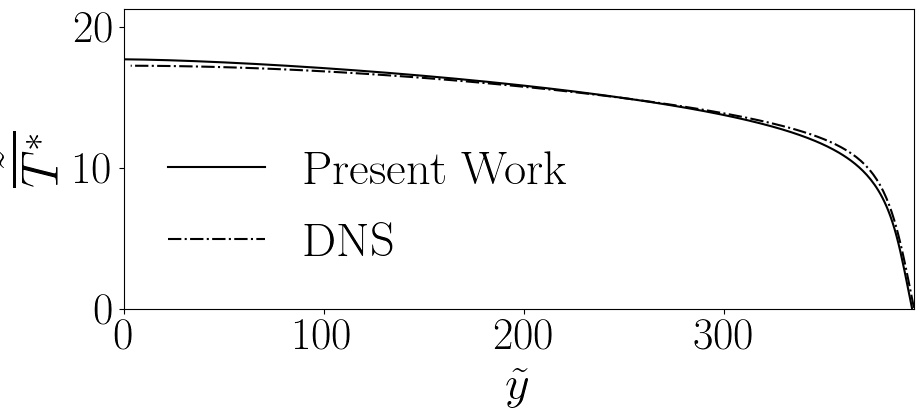
\includegraphics[angle=0, scale=0.34]{fotos_formatacao_final/Temperature_395_071_Prt0905_A26}
		\subcaption{$Re_\tau = 395$, $L2_t = 0.23$}
	\end{minipage}
	\begin{minipage}[t]{0.5\textwidth}
		\centering
		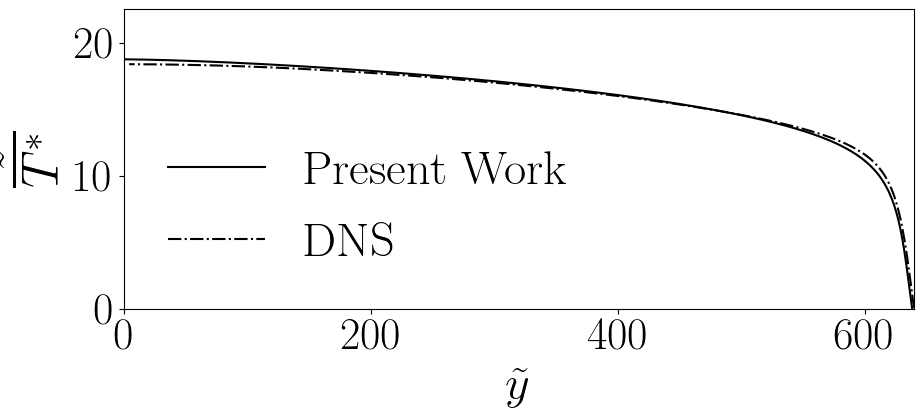
\includegraphics[angle=0, scale=0.34]{fotos_formatacao_final/Temperature_640_071_Prt0905_A26}
		\subcaption{$Re_\tau = 640$, $L2_t = 0.19$}
	\end{minipage}
	\begin{minipage}[t]{0.45\textwidth}
		\centering
		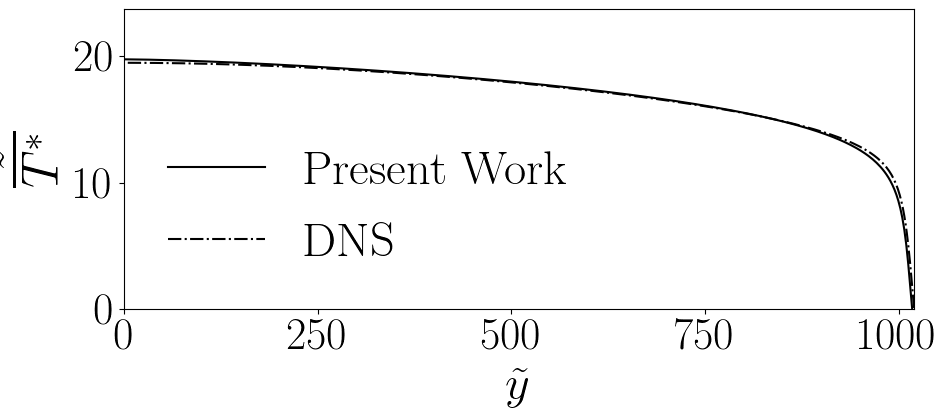
\includegraphics[angle=0, scale=0.34]{fotos_formatacao_final/Temperature_1000_071_Prt0905_A26}
		\subcaption{$Re_\tau = 1020$, $L2_t = 0.14$}
	\end{minipage}	
	\caption{Perfis de temperatura para simulações com $Pr_t = 0.9 $, $A = 26$ e $Pr =0.71$ }
	\label{primeiros}
\end{figure*}

Apesar de os resultados serem melhores, se comparados aos da figura \ref{figuraresultados1}, ainda havia mais espaço para melhoras. O número de Prandtl turbulento varia com o número de Reynolds turbulento, como pode ser visto em fig.\ref{figure5}, então um modelo que leve em conta a grandeza estaria mais próximo do correto. 
Para se obter a curva de $Pr_t$ em função do $Re_\tau$, o mesmo algorítmo foi usado, obtendo-se um valor de número de Prandtl turbulento ideal para cada número de Reynolds turbulento disponível resultados de DNS (\cite{dns1020} and \cite{dns150}).

Os valores obtidos podem ser conferidos na tabela \ref{tabela1}:

\begin{table}[!h]
	\centering
	\caption{Números de prandtl turbulentos ideais ajustados para cada número de Reynolds turbulento, com a constante de cebeci $A = 26$.}
	\begin{tabular}{ll}
		  \hline
		  $Re_\tau$ & $Pr_t$\\
		  \hline
		  150  &   0.94531\\
		  395  &   0.89531\\
		  640  &   0.89531\\
		  1020 &   0.90000\\ 
		  \hline
	\end{tabular}
	\label{tabela1}
\end{table}

Realizando um ajuste de curva polinomial, um modelo ajustado para o número de prandtl turbulento em função do número de reynolds foi desenvolvido:

\begin{equation}
  \begin{split}
    Pr_t = -4.5604 * 10^{-10} Re_\tau^3 + 9.5690 * 10^{-7} Re_\tau^2 - 6.1715 *10 ^{-4} Re_\tau + 1.0178 .
  \end{split}
\end{equation}

Os resultados das simulações foram muito acurados, ainda mais do que as simulações com os números turbulentos de prandtl definidos como valores médios dos dados dns (fig.\ref{figure5}). Estes resultados podem ser observados na figura \ref{figura_9}:

\begin{figure*}[!h]
	\centering
	\begin{minipage}[t]{0.5\textwidth}
		\centering
		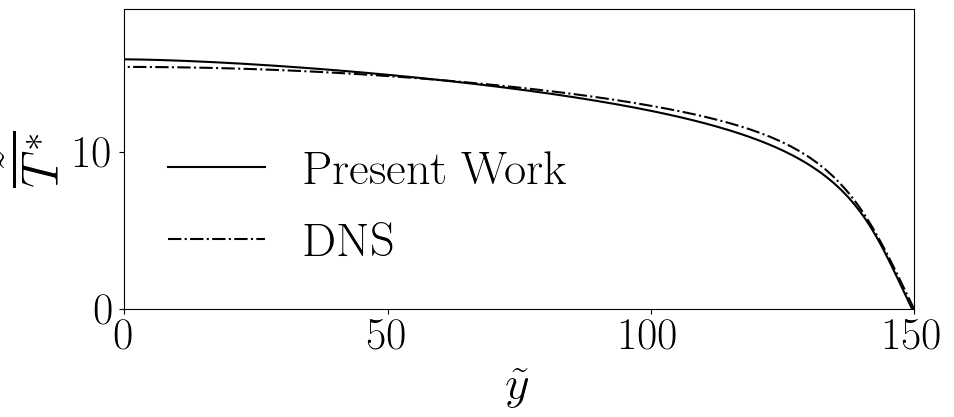
\includegraphics[angle=0, scale=0.34]{fotos_formatacao_final/Temperature_150_071_Prt(Ret)_A26}
		\subcaption{$Re_\tau = 150$, $L2_t = 0.26$}
	\end{minipage}
	\begin{minipage}[t]{0.45\textwidth}
		\centering
		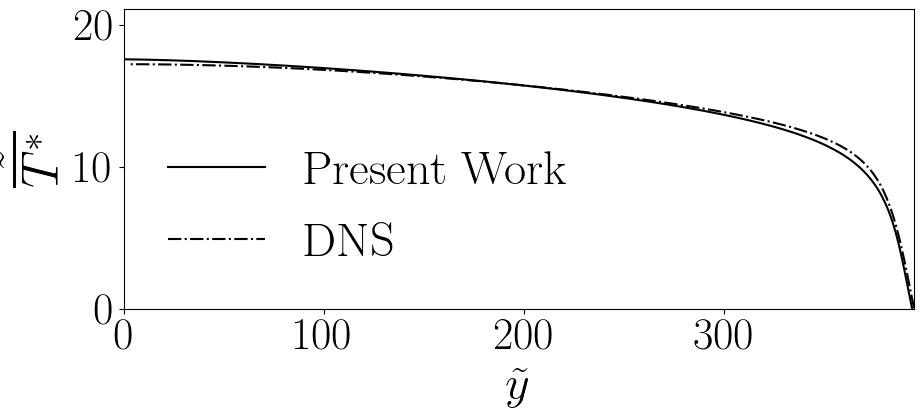
\includegraphics[angle=0, scale=0.34]{fotos_formatacao_final/Temperature_395_071_Prt(Ret)_A26}
		\subcaption{$Re_\tau = 395$, $L2_t = 0.22$}
	\end{minipage}
	\begin{minipage}[t]{0.5\textwidth}
		\centering
		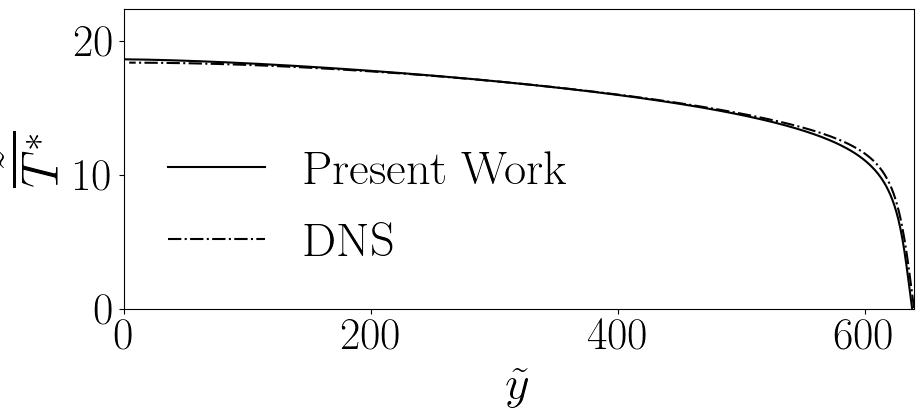
\includegraphics[angle=0, scale=0.34]{fotos_formatacao_final/Temperature_640_071_Prt(Ret)_A26}
		\subcaption{$Re_\tau = 640$, $L2_t = 0.17$}
	\end{minipage}
	\begin{minipage}[t]{0.45\textwidth}
		\centering
		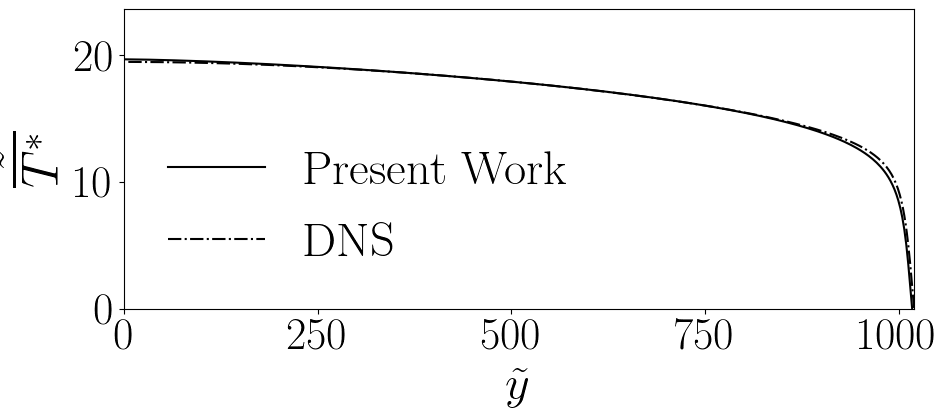
\includegraphics[angle=0, scale=0.34]{fotos_formatacao_final/Temperature_1000_071_Prt(Ret)_A26}
		\subcaption{$Re_\tau = 1020$, $L2_t = 0.14$}
	\end{minipage}	
	\caption{Resultados de temperatura para $Pr_\tau(Re_\tau)$, $A = 26$ e $Pr =0.71$. }
	\label{figura_9}
\end{figure*}

Outras formas de diminuir os erros foram buscadas. O perfil de velocidade era uma possibilidade, pois desempenha um papel importante no erro do método. Foram realizadas simulações desenvolvendo apenas esta propriedade física, e também houve erro associado (fig.\ref{figura_10}).

\begin{figure*}[!h]
	\centering
	\begin{minipage}[t]{0.5\textwidth}
		\centering
		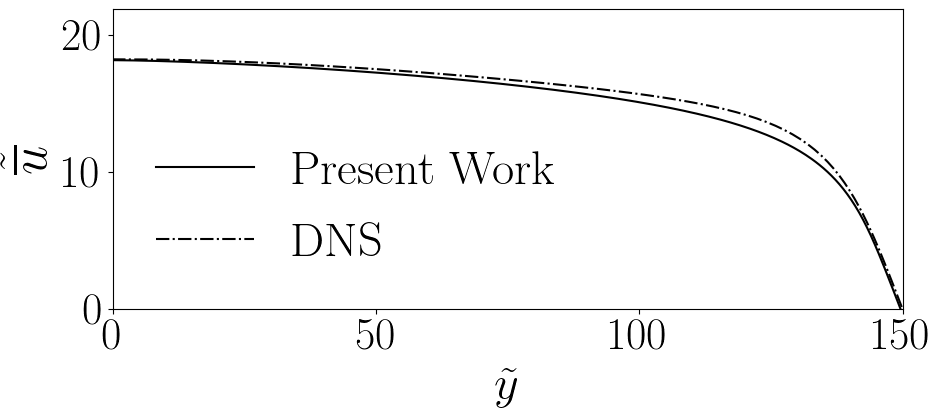
\includegraphics[angle=0, scale=0.34]{fotos_formatacao_final/Temperature_150_Avelocity}
		\subcaption{$Re_\tau = 150$, $L2_d = 0.47$}
	\end{minipage}
	\begin{minipage}[t]{0.45\textwidth}
		\centering
		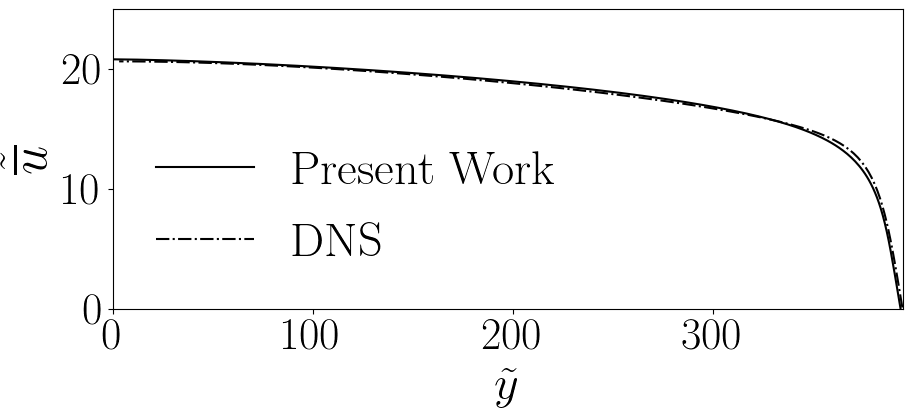
\includegraphics[angle=0, scale=0.34]{fotos_formatacao_final/Temperature_395_Avelocity}
		\subcaption{$Re_\tau = 395$, $L2_d = 0.17$}
	\end{minipage}
	\begin{minipage}[t]{0.5\textwidth}
		\centering
		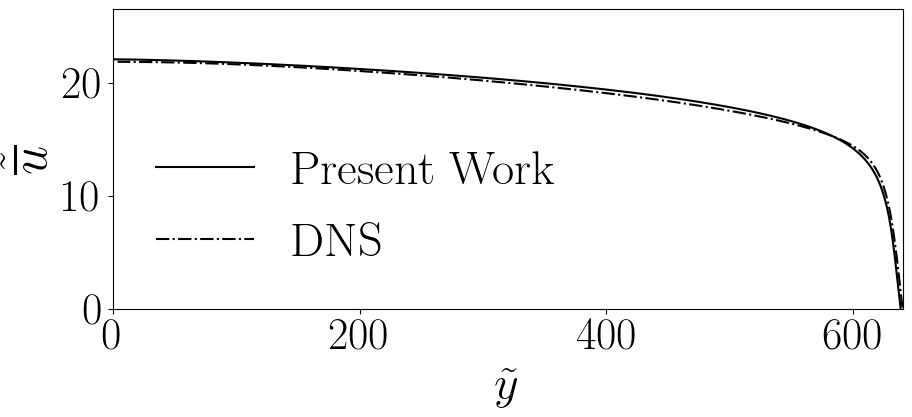
\includegraphics[angle=0, scale=0.34]{fotos_formatacao_final/Temperature_640_Avelocity}
		\subcaption{$Re_\tau = 640$, $L2_d = 0.23$}
	\end{minipage}
	\begin{minipage}[t]{0.45\textwidth}
		\centering
		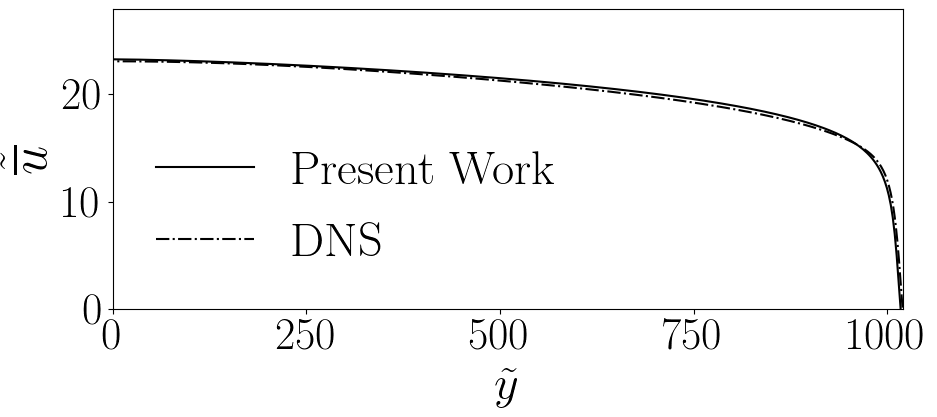
\includegraphics[angle=0, scale=0.34]{fotos_formatacao_final/Temperature_1000_Avelocity}
		\subcaption{$Re_\tau = 1020$, $L2_d = 0.23$}
	\end{minipage}	
	\caption{Resultados de perfil de velocidade para $A = 26$.}
	\label{figura_10}
\end{figure*}

Um modelo ajustado foi proposto no presente trabalho para a constante de cebeci, $A$, com o objetivo de redução no erro. O mesmo algorítmo usado para se achar o número de prandtl turbulento ideal foi utilizado para se encontrar a constante de Cebeci ideal. A velocidade do DNS foi utilizada para o cálculo do erro (norma L2).

Os resulados para a constante de Cebeci ideal são apresentados na tabela \ref{tablea}:

\begin{table}[!h]
	\centering
	\caption{Constante de Cebeci ideal ajustada para cada número de Reynolds turbulento.}
	\begin{tabular}{ll}
		\hline
		$Re_\tau$ & $A$\\
		\hline
		150  &   28.616180\\
		395  &   25.673782\\
		640  &   25.001266\\
		1020 &   25.002136\\ 
		\hline
	\end{tabular}
	\label{tablea}
\end{table}

Foi possível observar que para altos valores de Reynolds, a constante se aproximou no valor canônico encontrado na literatura, enquanto para baixos valores de número de Reynolds turbulento houve grande divergência.

Dessa forma, com os pontos encontrados e listados na tabela, foi possível realizar um encaixe de curva para se encontrar a função que fornece o número de Cebeci ideal a partir do número de Reynolds turbulento.

A partir destes resultados foi possível a criação de um modelo para a constante de Cebeci, que pode ser visto na equação que segue:

\begin{equation}\label{Amodelado}
A \left( Re_\tau\right)= \frac{Re_\tau ^{0.0451 * \ln(Re_\tau)} *e ^ {5.2753} }{Re_\tau ^{0.6094}}.
\end{equation}

Assim, a partir destes novos valores de Cebeci ajustados, foi possível o desenvolvimento de simulações de velocidade mais acuradas como se pode ver nos resultados que seguem:

\begin{figure*}[!h]
	\centering
	\begin{minipage}[t]{0.5\textwidth}
		\centering
		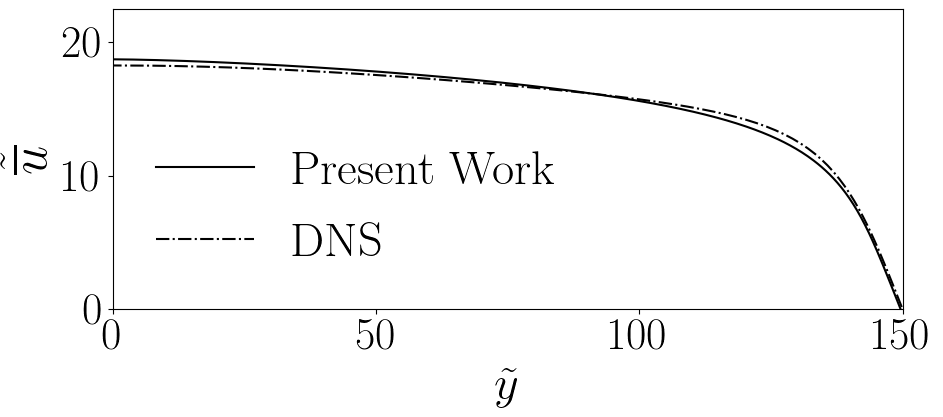
\includegraphics[angle=0, scale=0.34]{fotos_formatacao_final/Temperature_150_Amodeled}
		\subcaption{$Re_\tau = 150$, $L2_d = 0.28$}
	\end{minipage}
	\begin{minipage}[t]{0.45\textwidth}
		\centering
		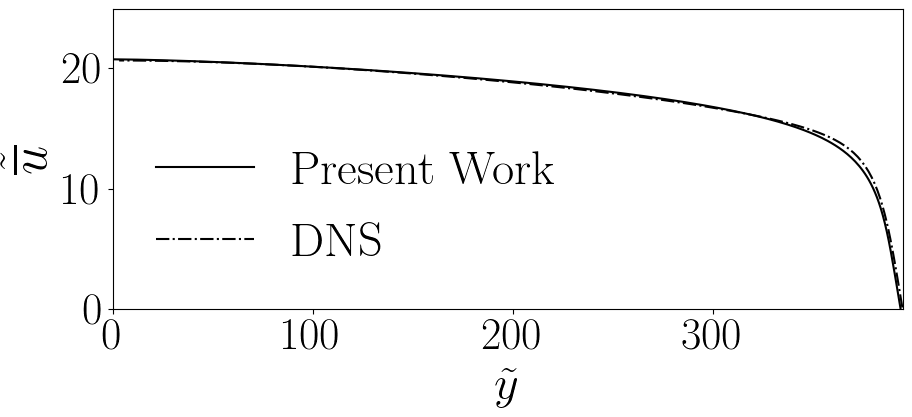
\includegraphics[angle=0, scale=0.34]{fotos_formatacao_final/Temperature_395_Amodeled}
		\subcaption{$Re_\tau = 395$, $L2_d = 0.16$}
	\end{minipage}
	\begin{minipage}[t]{0.5\textwidth}
		\centering
		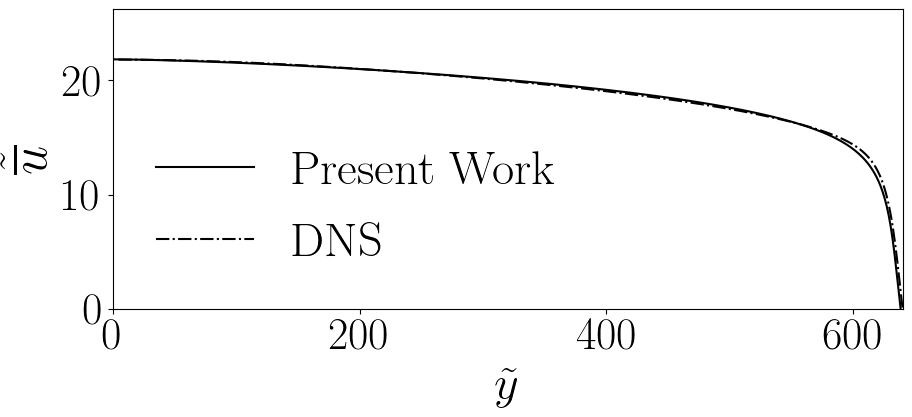
\includegraphics[angle=0, scale=0.34]{fotos_formatacao_final/Temperature_640_Amodeled}
		\subcaption{$Re_\tau = 640$, $L2_d = 0.14$}
	\end{minipage}
	\begin{minipage}[t]{0.45\textwidth}
		\centering
		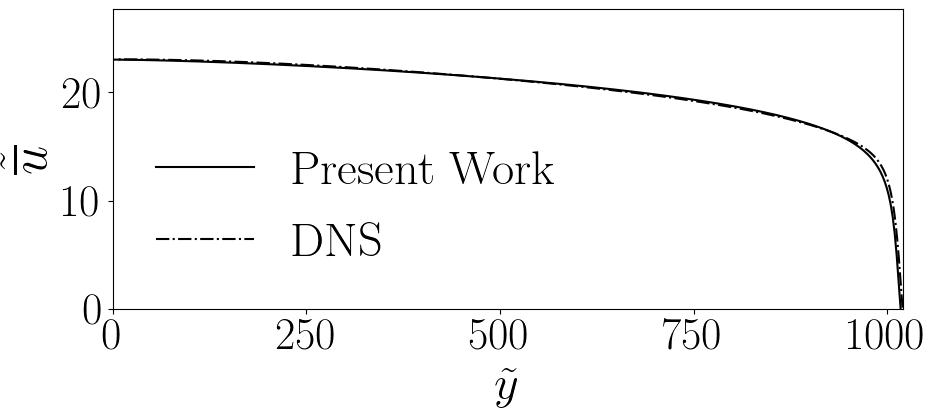
\includegraphics[angle=0, scale=0.34]{fotos_formatacao_final/Temperature_1000_Amodeled}
		\subcaption{$Re_\tau = 1020$, $L2_d = 0.13$}
	\end{minipage}	
	\caption{Resultados em distribuição de velocidade para o modelo de A \ref{Amodelado}.}
\end{figure*}

Com a função de Cebeci ajustada, um novo grupo de otimizações foi feito, com a mesma metodologia de evolução diferencial, levando em consideração esta nova formulação para a constante de cebeci. Tal estudo resultou em um novo conjunto de número de prandtl turbulento ótimo para cada número de 
Reynolds turbulento, como segue:

\begin{table}[!h]
	\centering
	\caption{Números de prandtl turbulentos ideais ajustados para cada número de Reynolds turbulento, com a função de Cebeci ajustada.}
	\begin{tabular}{ll}
		\hline
		$Re_\tau$ & $Pr_t$\\
		\hline
		150  &   0.88594\\
		395  &   0.90156\\
		640  &   0.91094\\
		1020 &   0.91406\\ 
		\hline
	\end{tabular}
\end{table}

Assim um novo modelo pode ser proposto para o número de Prandtl turbulento:

\begin{equation}
  \begin{split}
    Pr_t = 4.5290 * 10^{-12} Re_\tau^3 - 5.7395 * 10^{-8} Re_\tau^2 + 9.397 * 10^{-5} Re_\tau + 0.8731.
  \end{split}
\end{equation}

\vspace{0.5cm}

Esse novo modelo pode ser considerado mais acurado, uma vez que ele foi desenvolvido minimizando-se os erros advindos da simulação térmica.

Com esta nova parametrização, uma nova série de simulações foram desenvolvidas para se obter a temperatura no canal:
   
\begin{figure*}[!h]
	\centering
	\begin{minipage}[t]{0.5\textwidth}
		\centering
		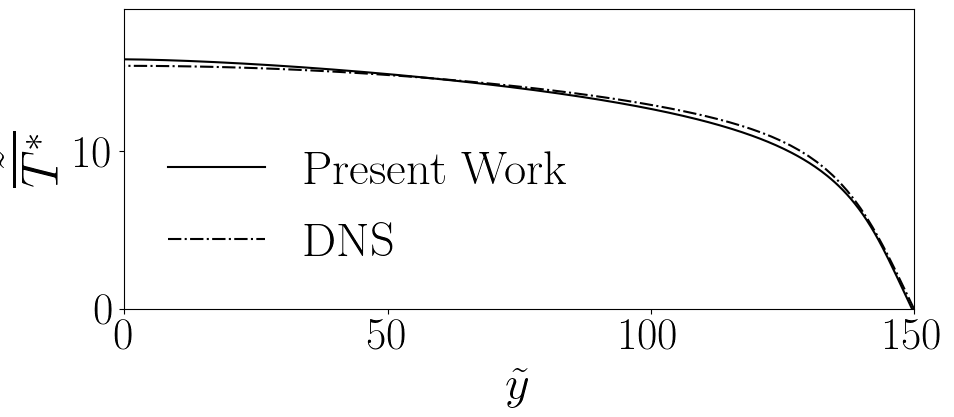
\includegraphics[angle=0, scale=0.34]{fotos_formatacao_final/Temperature_150_071_Prt(Ret)_Avelocity}
		\subcaption{$Re_\tau = 150$, $L2_t = 0.212$}
	\end{minipage}
	\begin{minipage}[t]{0.45\textwidth}
		\centering
		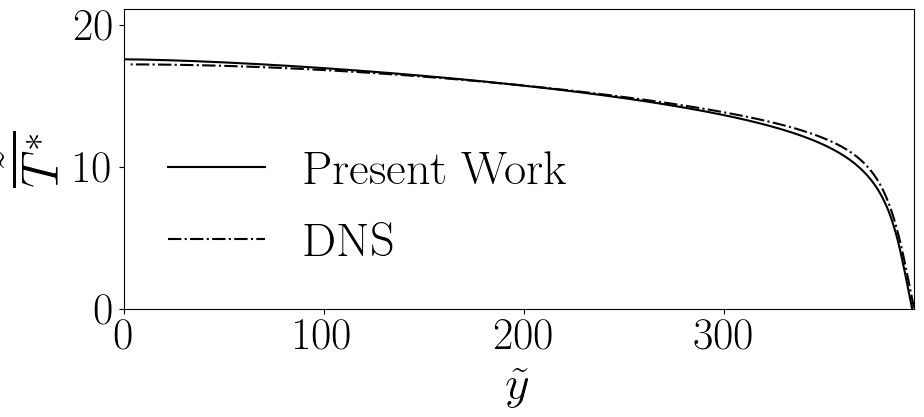
\includegraphics[angle=0, scale=0.34]{fotos_formatacao_final/Temperature_395_071_Prt(Ret)_Avelocity}
		\subcaption{$Re_\tau = 395$, $L2_t = 0.233$}
	\end{minipage}
	\begin{minipage}[t]{0.5\textwidth}
		\centering
		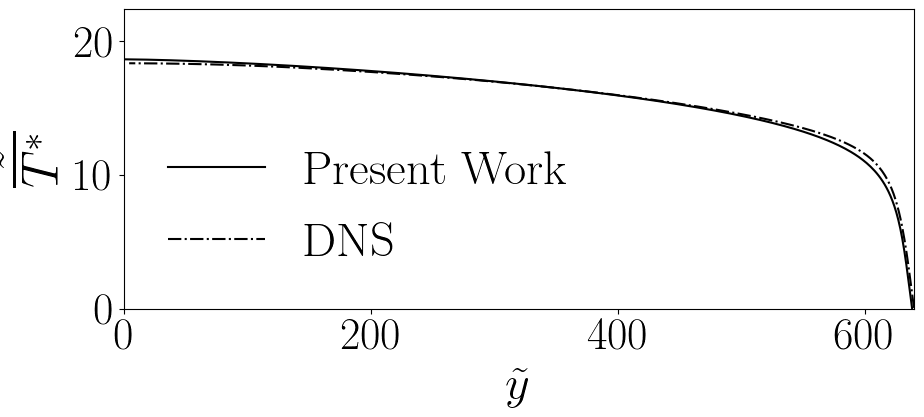
\includegraphics[angle=0, scale=0.34]{fotos_formatacao_final/Temperature_640_071_Prt(Ret)_Avelocity}
		\subcaption{$Re_\tau = 640$, $L2_t = 0.205$}
	\end{minipage}
	\begin{minipage}[t]{0.45\textwidth}
		\centering
		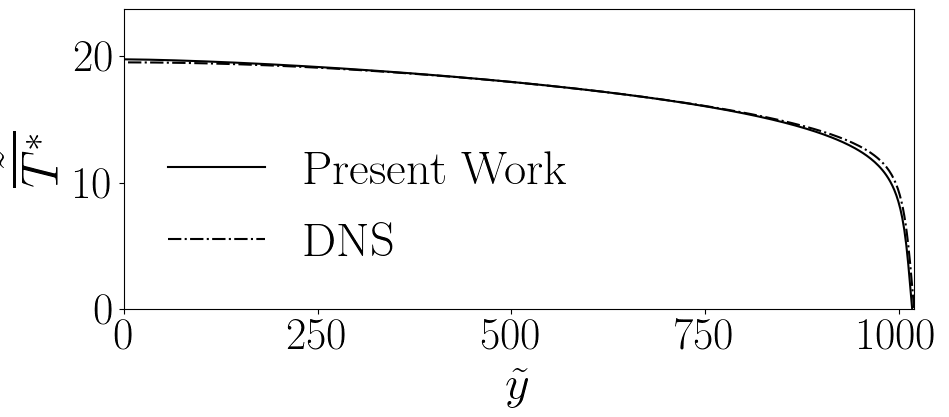
\includegraphics[angle=0, scale=0.34]{fotos_formatacao_final/Temperature_1000_071_Prt(Ret)_Avelocity}
		\subcaption{$Re_\tau = 1020$, $L2_t = 0.175$}
	\end{minipage}	
	\caption{Resultados térmicos para $Pr_\tau(Re\tau)$, $A(Re_\tau)$ e $Pr =0.71$ }
\end{figure*}

Os valores de Cebeci que resularam em um erro menor para a velocidade não tiveram o mesmo efeito na temperatura. Do ponto de vista algébrico, a constante de Cebeci aparece duas vezes: sob um contexto térmico e sob um contexto dinâmico (\ref{equationultima} e \ref{finalequationvelocity}).

Então, como última tentativa de melhorar o modelo, foi feita uma nova otimização, dessa vez, considerando a constante de Cebeci de forma separada no contexto da temperatura ($A_t$) e no contexto da velocidade ($A_d$).

Outro método de ajuste a partir de evolução diferencial é o ajuste multiobjetivo. Tal abordagem foi utilizada para considerar mais de uma variável para edição simultaneamente durante a otimização. Este método foi usado para ajustar a função térmica de cebeci e o número de Prandtl turbulento para o menor erro (norma L2) no campo de temperatura resultante para cada amostra DNS. A função cebeci para velocidade foi considerada no desenvolvimento anterior. Novos valores ideais foram encontrados para o número de Prandtl turbulento e a constante de cebeci térmica:

\begin{table}[!h]
	\centering
	\caption{Números de prandtl turbulentos ideais e função de cebeci térmica ($A_t$) ajustados para cada número de Reynolds turbulento, com a abordagem multiobjetiva.}
	\begin{tabular}{llll}
		\hline
		$Re_\tau$ & $Pr_t$ & $A_t$ & $A_d$\\
		\hline
		150  &   0.72530 & 37.25510 & 28.616180\\
		395  &   0.76821 & 34.24176 & 25.673782\\
		640  &   0.81896 & 31.27627 & 25.001266\\
		1020 &   0.86179 & 28.73726 & 25.002136\\ 
		\hline
	\end{tabular}
\end{table}

Com tais dados numéricos, novos modelos foram propostos para o número de prandtl turbulento e a função de cebeci termal:

\begin{equation}
  A_t = \frac{Re_\tau ^{0.0395 \ln(Re_\tau)^2 - 0.7588 \ln(Re_\tau) +  4.6637  } }{e ^{5.6703}},
\end{equation}

\begin{equation}
  \begin{split}
    Pr_t = -2.4892 * 10^{-10} Re_\tau^3 +  3.6036 * 10^{-7} Re_\tau^2 + 3.7921 *10 ^{-5} Re_\tau + 0.7123 .
  \end{split}
\end{equation}

Novas simulações foram feitas usando os novos modelos propostos:

\begin{figure*}[!h]
	\centering
	\begin{minipage}[t]{0.5\textwidth}
		\centering
		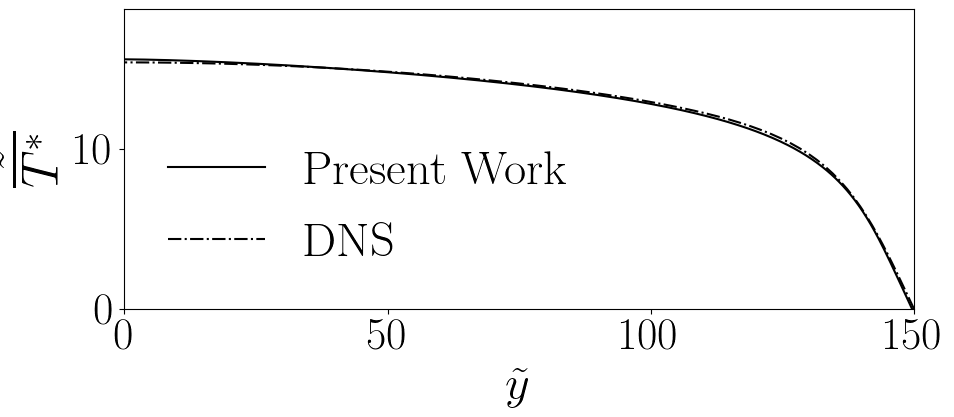
\includegraphics[angle=0, scale=0.24]{fotos_formatacao_final/Temperature_150_071_Genetic2temperature}
		\subcaption{$Re_\tau = 150$, $L2_t = 0.091$}
	\end{minipage}
	\begin{minipage}[t]{0.45\textwidth}
		\centering
		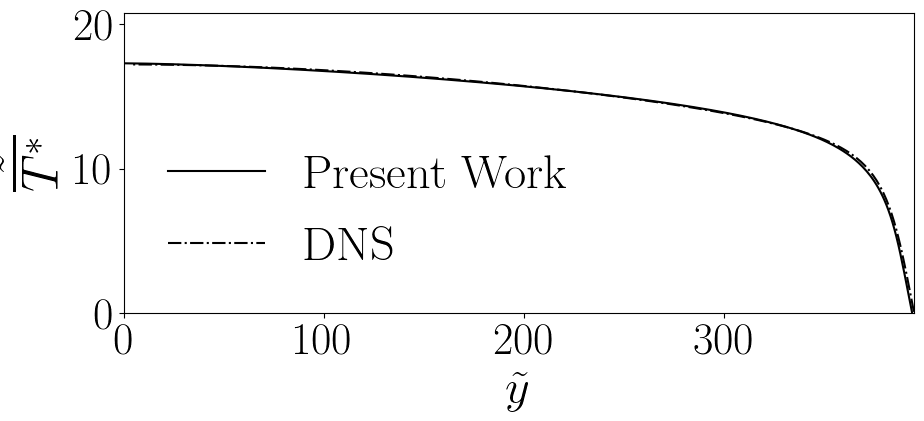
\includegraphics[angle=0, scale=0.24]{fotos_formatacao_final/Temperature_395_071_Genetic2temperature}
		\subcaption{$Re_\tau = 395$, $L2_t = 0.049$}
	\end{minipage}
	\begin{minipage}[t]{0.5\textwidth}
		\centering
		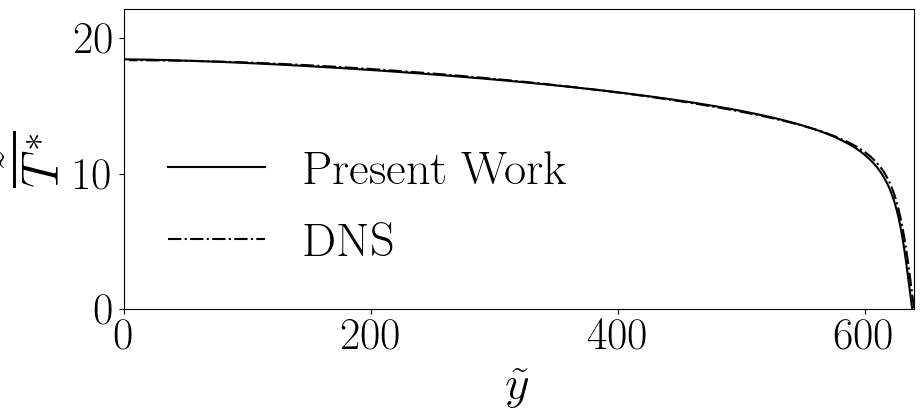
\includegraphics[angle=0, scale=0.24]{fotos_formatacao_final/Temperature_640_071_Genetic2temperature}
		\subcaption{$Re_\tau = 640$, $L2_t = 0.061$}
	\end{minipage}
	\begin{minipage}[t]{0.45\textwidth}
		\centering
		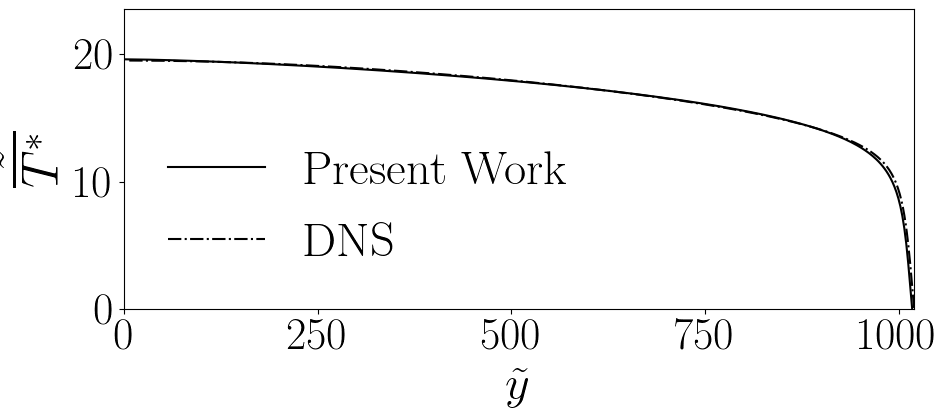
\includegraphics[angle=0, scale=0.24]{fotos_formatacao_final/Temperature_1000_071_Genetic2temperature}
		\subcaption{$Re_\tau = 1020$, $L2_t = 0.076$}
	\end{minipage}	
	\caption{Results of temperature simulations for $Pr_\tau(Re_\tau)$, $A_d(Re_\tau)$, $A_t(Re_\tau) $ and $Pr =0.71$, with multi-objective adjustment.}
\end{figure*}

Estes foram os melhores resultados obtidos.


\chapter{Simulações no MFsim}

Tendo-se estes novo modelos sido propostos, novas simulações foram feitas no MFsim, visando validar se estes modelos para a constante de Cebeci e o número de Prandtl turbulento tem utilidade em softwares comerciais de simulação fluidodinâmica.

\section{Sobre a parametrização do sistema}
Estabeleceu-se o domínio computacional como um paralelepípedo de dimensões $0.25m$ por $0.25m$ por $2m$, onde a dimensão maior seria a no sentido da corrente. A partir disso, calculou-se o gradiente de pressão a partir das seguintes equações:

\begin{equation}
  Re_\tau = \frac{u_\tau R}{\nu}
\end{equation}

\begin{equation}
  u_\tau = \sqrt{\frac{|\tau_w|}{\rho}}
\end{equation}

\begin{equation}
  \tau_w = \Delta P \frac{R}{L}
\end{equation}

Desenvolvimendo as equações acima, tem-se:

\begin{equation}
  \Delta P = \tau_w \frac{L}{R}
\end{equation}

\begin{equation}
  \tau_w = \rho u_\tau^2
\end{equation}

\begin{equation}
  u_\tau = \frac{\nu Re_\tau}{R}
\end{equation}


Assim, esbosa-se uma relação entre a diferença de pressão e o número de Reynolds:

\begin{equation}
  \Delta P = Re_\tau^2 \frac{L \mu^2}{\rho R^3}
\end{equation}

\begin{equation}
  \Delta P =3 Re \frac{L \mu^2}{\rho R^2}
\end{equation}

Adotam-se os seguintes valores:
\begin{itemize}
  \item $L = 2m$
  \item $R = 0.125m$
  \item $\mu = 0.1 kg/m.s$
  \item $\rho = 100 kg/m^3$
\end{itemize}

A partir destas equações é possível se calcular o valor da diferença de pressão entre a entrada e saída do fluxo a partir do número de Raynolds avaliado, segue uma tabela com os valores de diferença de pressão resultantes:

\begin{table}[!h]
  \centering
  \caption{Valores de diferença de pressão para cada número de Reynolds turbulento.}
  \begin{tabular}{ll}
    \hline
    $Re_\tau$ & $\Delta P$ \\
    \hline
    150  &   2304 &
    395  &   15976,96 &
    640  &   41943,04 &
    1020 &   106536,96 &
    \hline
  \end{tabular}
\end{table}

\section{O domínio computacional}
Assim, para representar o domínio, uma malha de $200$ volumes por $25$ volumes por $25$ volumes. O que resultou em volumes cúbicos de $0.01cm$ de tamanho. A malha gerada pode ser vista na figura \ref{fig:malha}:

\begin{figure}[!h]
  \centering
  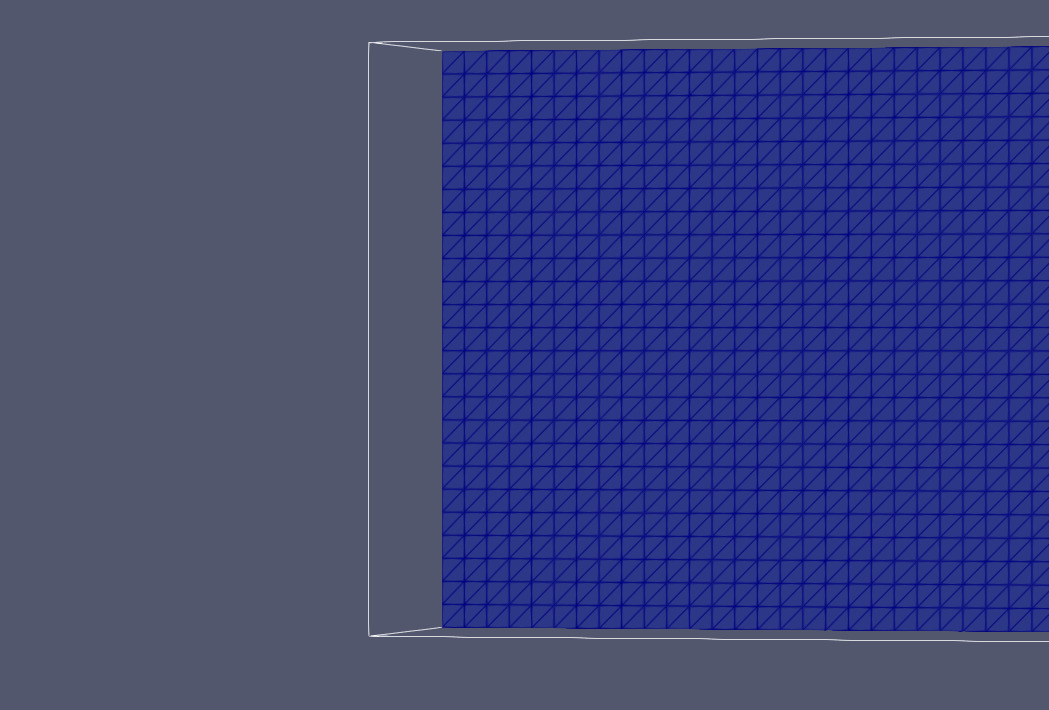
\includegraphics[angle=0, scale=0.25]{cap_fundamentacao/domain_mesh.jpeg}
  \caption{Malha gerada para a simulação.}
  \label{fig:malha}
\end{figure}

Para a condição de contorno estipulou-se dirichlet para a presão nas paredes perpendiculares ao eixo $x$ (no sentido da corrente), a partir dos valores caluclados anteriormente, assim como nas paredes perpendiculares ao eixo $z$, enquanto as velocidades foram mantidas como newmann, considerando-se auto similaridade no eixo $z$. Já nas paredes perpendiculares ao eixo $y$, configuraram-se as velocidades iqual a zero, uma vez que é onde estão localizadas as paredes em condição de não escorregamento. Os resultados iniciais podem ser vistos adiante (\ref{fig:first_results}):

\begin{figure}[!h]
  \centering
  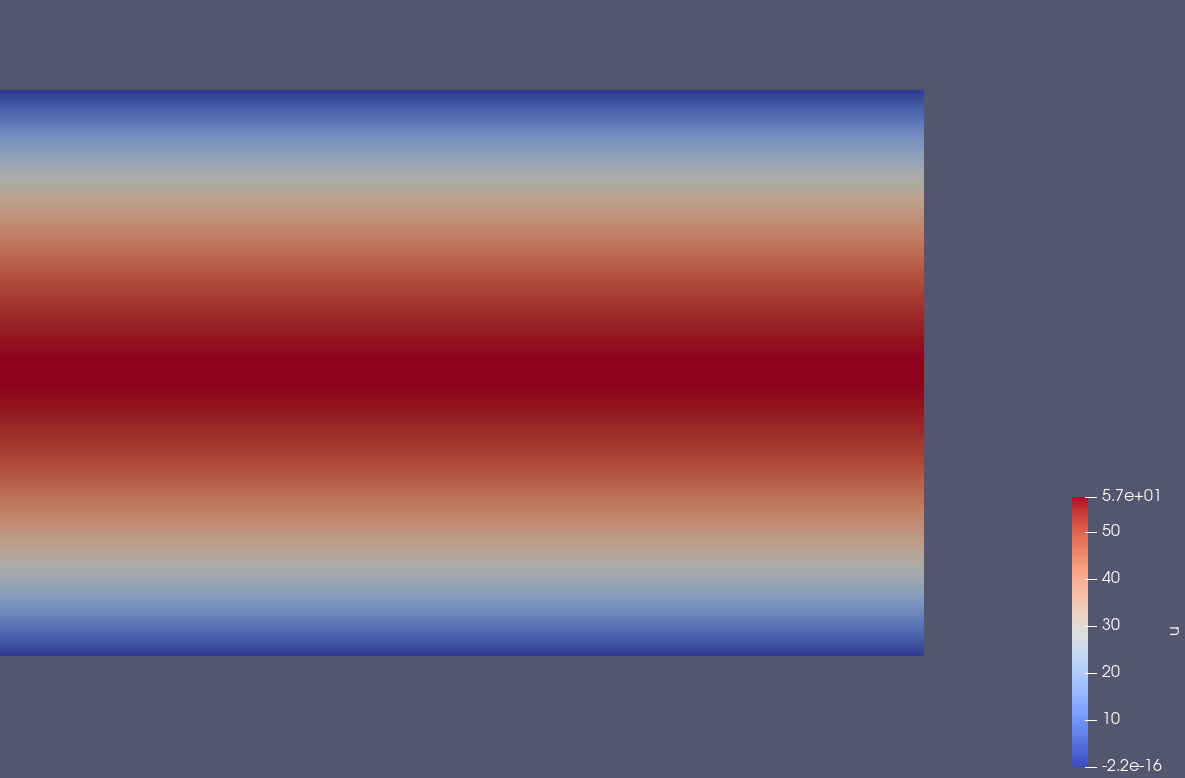
\includegraphics[angle=0, scale=0.25]{cap_fundamentacao/first_results.png}
  \caption{Resultados para $Re_\tau = 150$.}
  \label{fig:first_results}
\end{figure}

Notou-se que a velocidade no meio do canal ficou próximo de $57 m/s$, que ao adimensionalizar ($\tilde{u} = \frac{u}{u_\tau}$ e $u_\tau = \frac{\mu Re_\tau}{\rho R}$) é igual a 47.5, que é bem distante do valor de velocidade calculado para os mesmos valores de constante de cebeci e número de prandtl turbulento, que deveria ser por volta de 18 m/s. Por se distanciar do DNS também, pode ser algo errado com a determinação do Reynolds turbulento.
